%%%%%%%%%%%%%%%%%%%%%%%%%%%%%%%%%%%%%%%%%%%%%%%%%%%%%%%%%%%%%%%%%
\chapter{UYGULAMA VE BULGULAR}\label{ch:bulgular}
%%%%%%%%%%%%%%%%%%%%%%%%%%%%%%%%%%%%%%%%%%%%%%%%%%%%%%%%%%%%%%%%%
\vspace*{-1cm}

Aura Finance uygulaması, geliştirilen mimari ve algoritmaların birleşimiyle tam fonksiyonel bir finansal yönetim platformu olarak hayata geçirilmiştir. Bu bölümde, uygulamanın kullanıcı arayüzü ve elde edilen bulgular ekran görüntüleri eşliğinde sunulmaktadır.

\section{Kullanıcı Arayüzü Analizi}

Uygulamanın arayüzü, kullanıcı deneyimini (UX) ön planda tutan modern bir yapıdadır.

\subsection{Gösterge Paneli (Dashboard)}
Şekil~\ref{fig:sc1}'de görülen ana ekran, kullanıcının o ayki toplam harcamasını, kalan bütçesini ve harcama trendlerini özetler. AI Insights bölümü burada canlı olarak güncellenir.

\begin{figure}[h!]
 \centering
 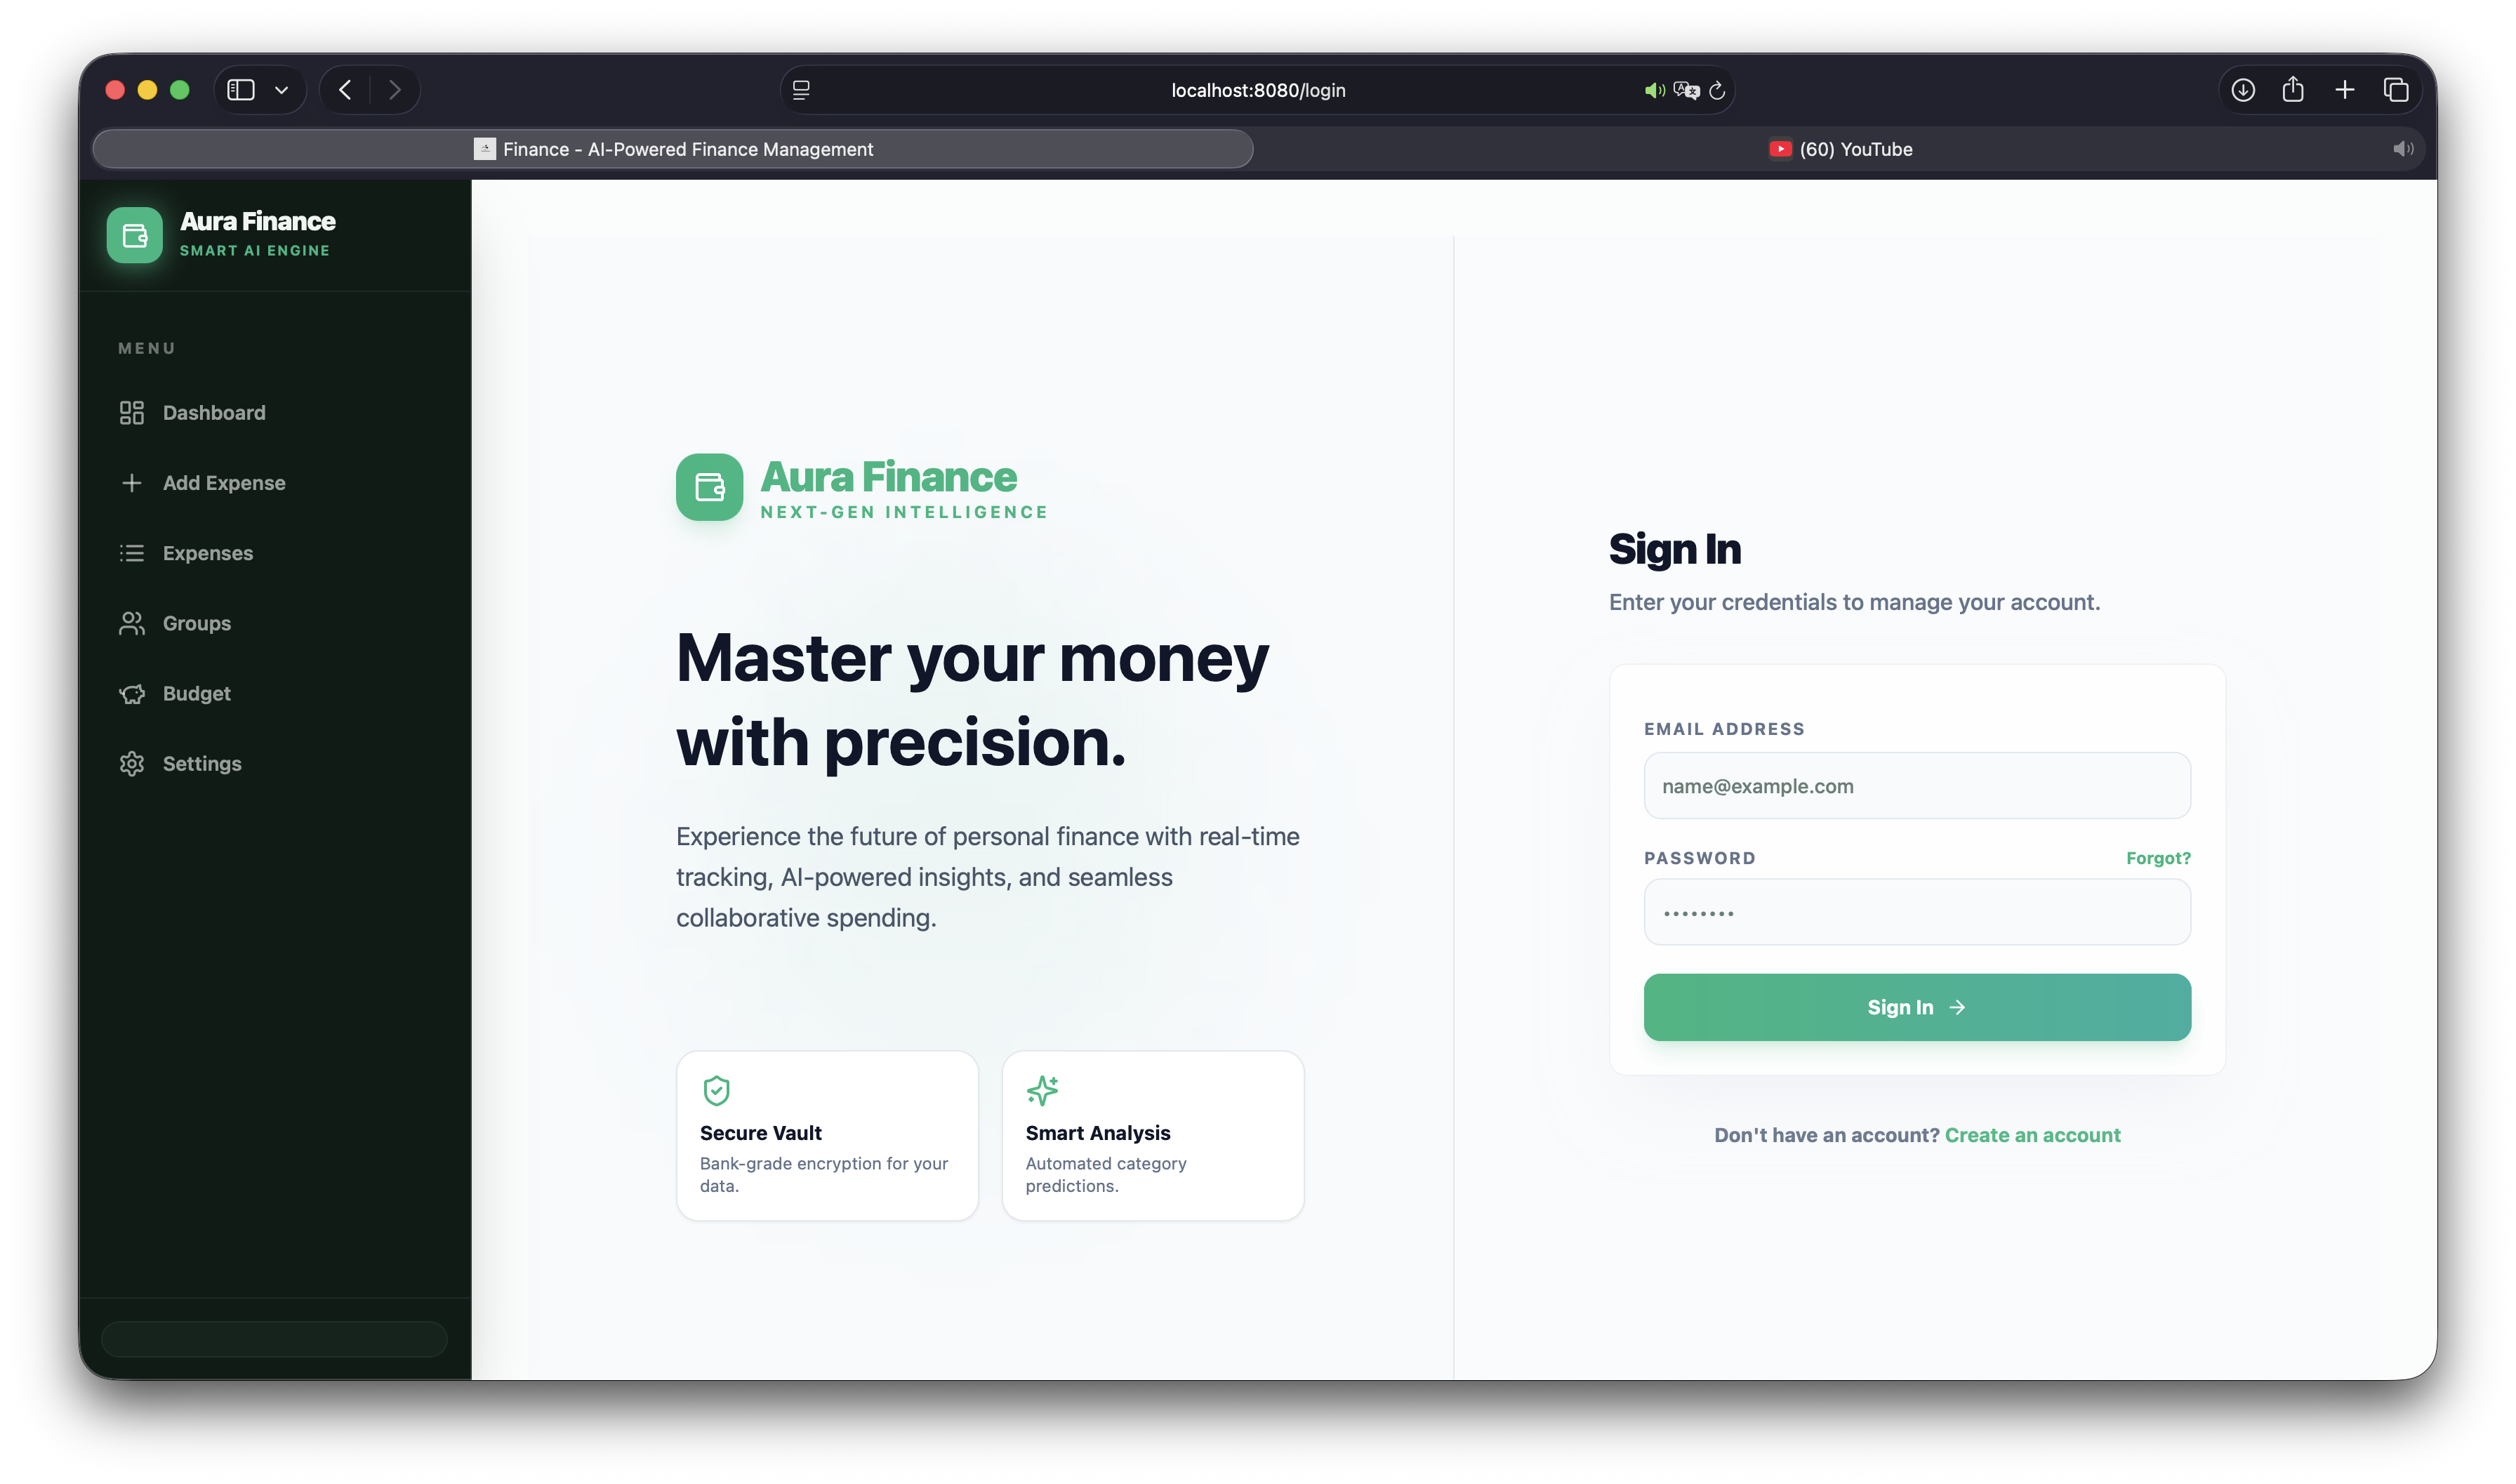
\includegraphics[width=0.8\textwidth]{./fig/aura_sc1}
 \caption{Aura Finance Gösterge Paneli ve Genel Bakış.}
 \label{fig:sc1}
\end{figure}

\subsection{Harcama Yönetimi}
Harcamaların listelendiği ve filtrelendiği ekran Şekil~\ref{fig:sc3}'te sunulmuştur. Kullanıcılar harcamalarını kategoriye, tarihe ve tutara göre sıralayabilmektedir.

\begin{figure}[h!]
 \centering
 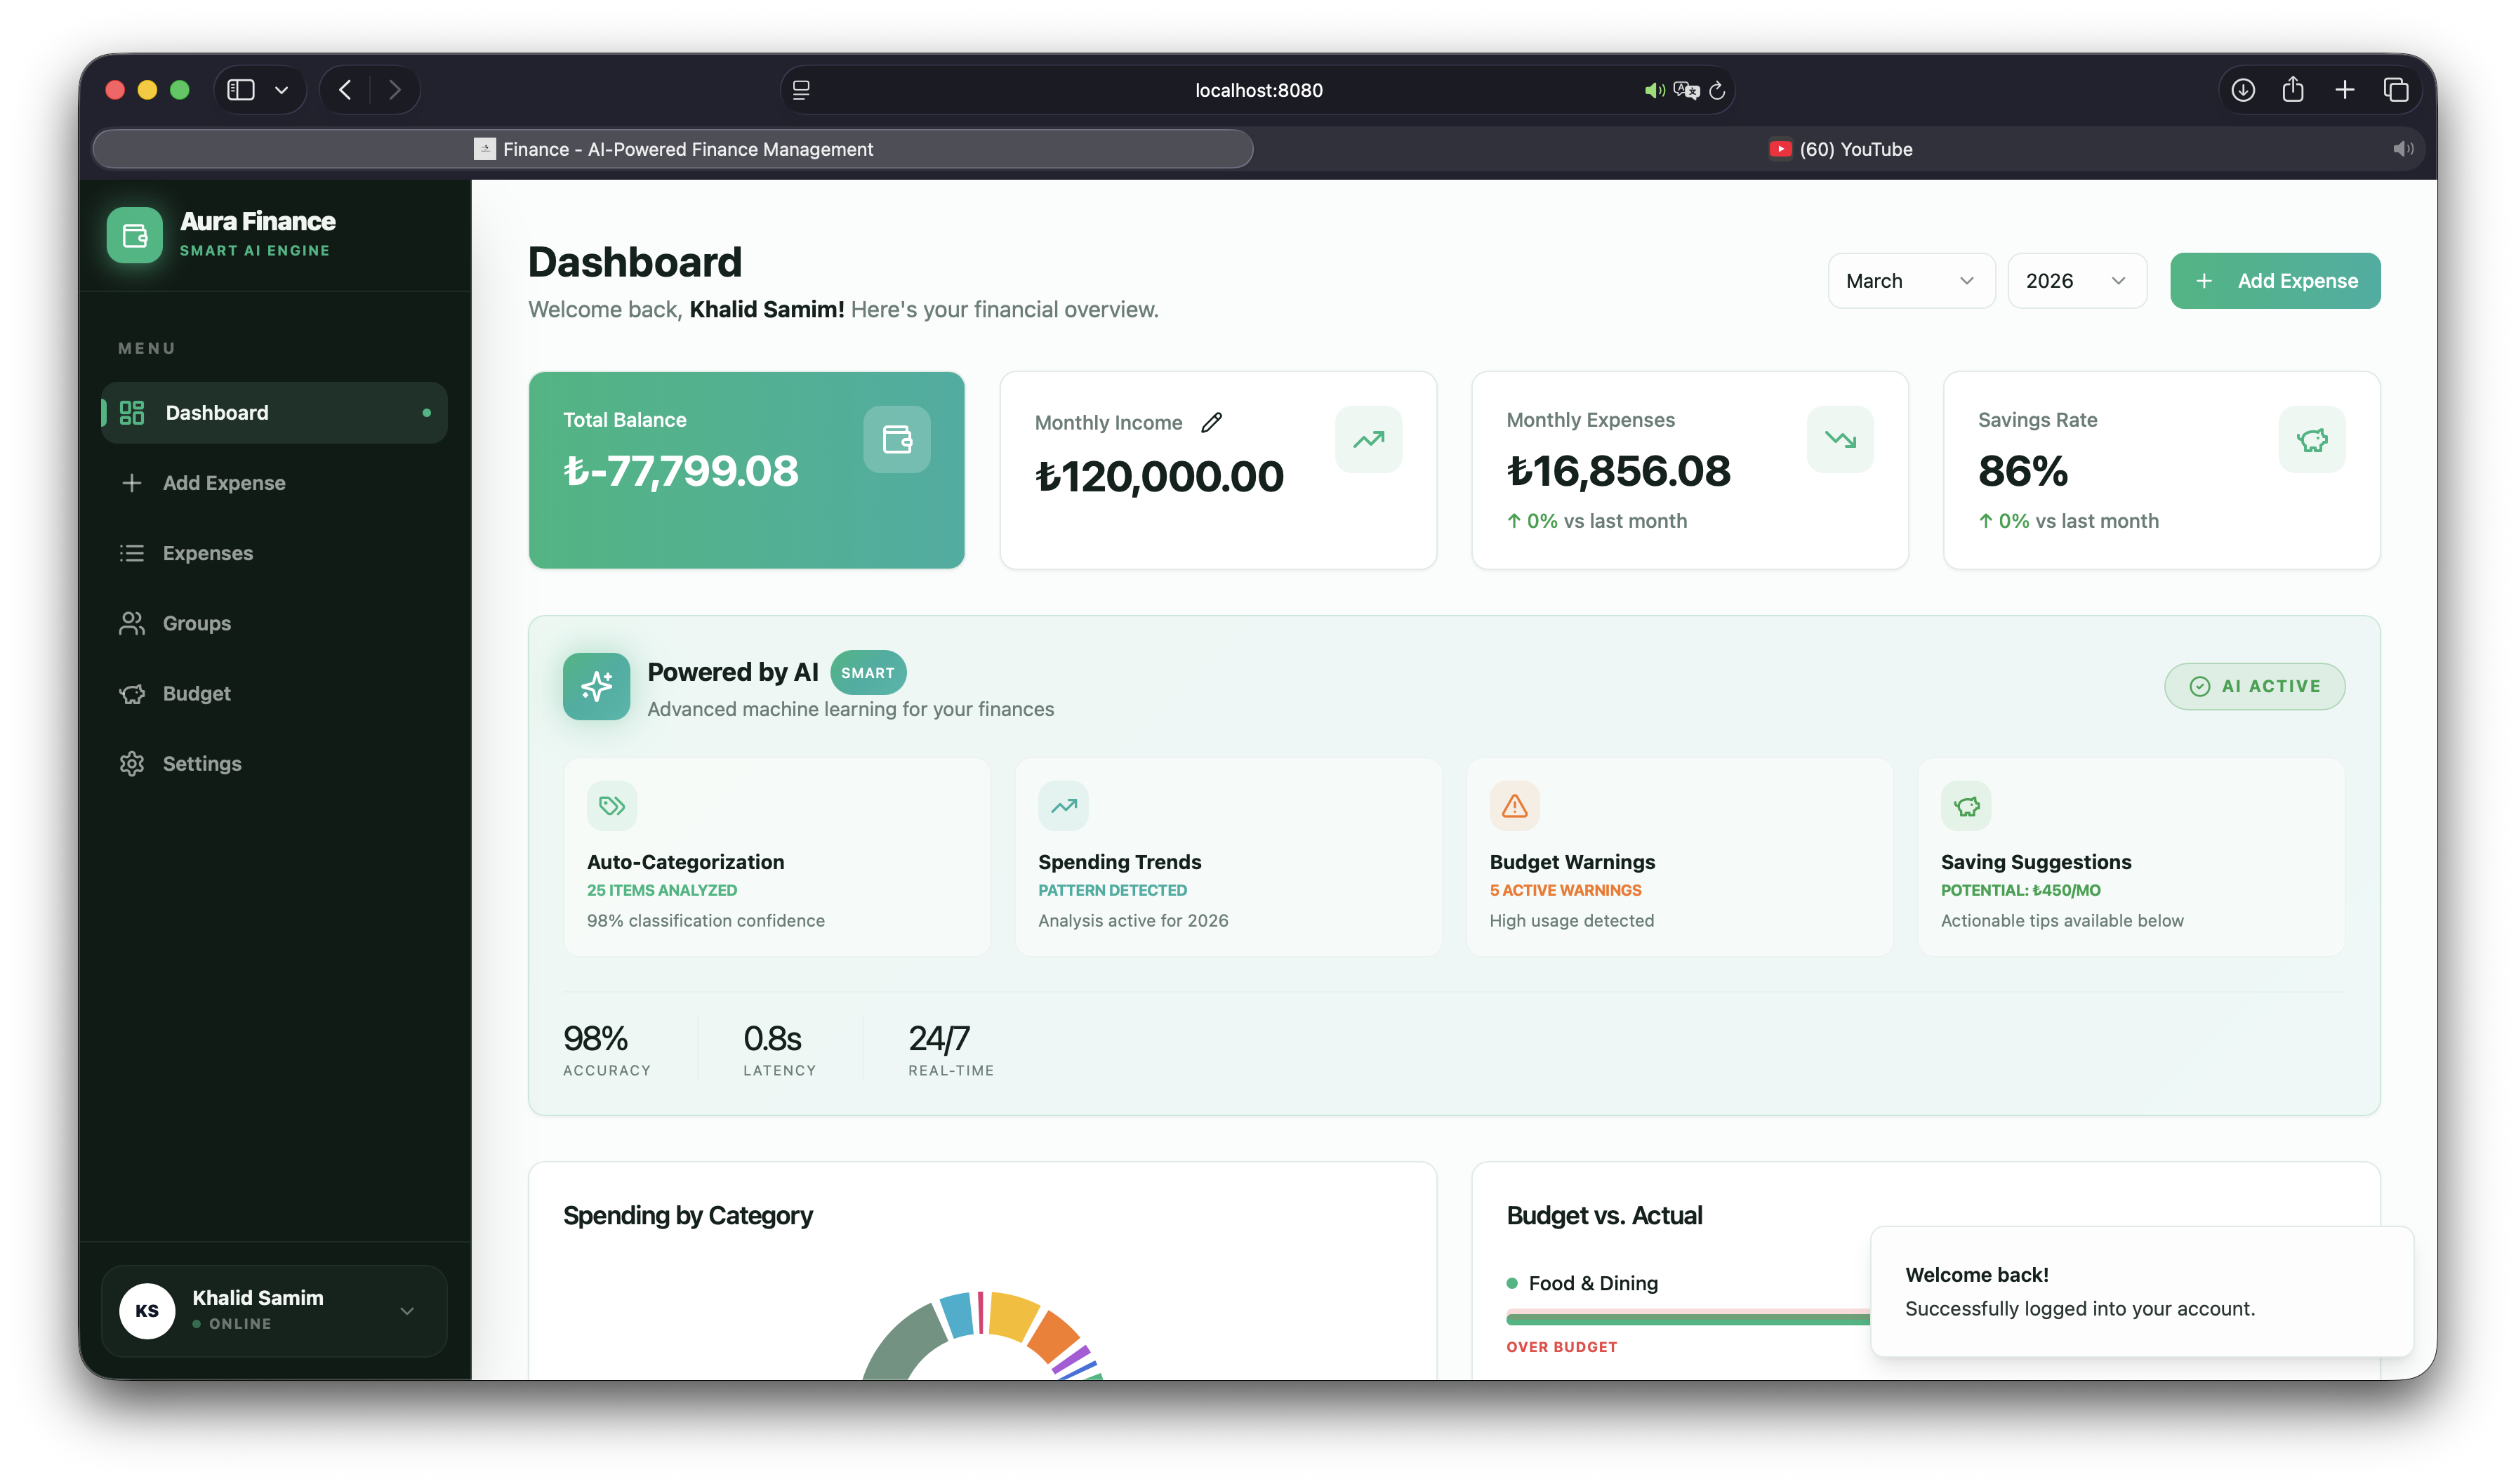
\includegraphics[width=0.8\textwidth]{./fig/aura_sc3}
 \caption{Harcama Listesi ve Filtreleme Seçenekleri.}
 \label{fig:sc3}
\end{figure}

\section{Yapay Zekâ ve Tahminleme Sonuçları}

Uygulamanın en kritik bileşeni olan tahminleme ve optimizasyon modülleri başarıyla çalışmaktadır.

\subsection{Zaman Serisi Tahmin Grafikleri}
Şekil~\ref{fig:sc10}'da görülen grafik, kullanıcının geçmiş harcama verilerine dayanarak LSTM modeli tarafından üretilen gelecek ay tahminlerini göstermektedir. Modelin güven aralığı verinin yoğunluğuna göre \%70 ile \%95 arasında değişmektedir.

\begin{figure}[h!]
 \centering
 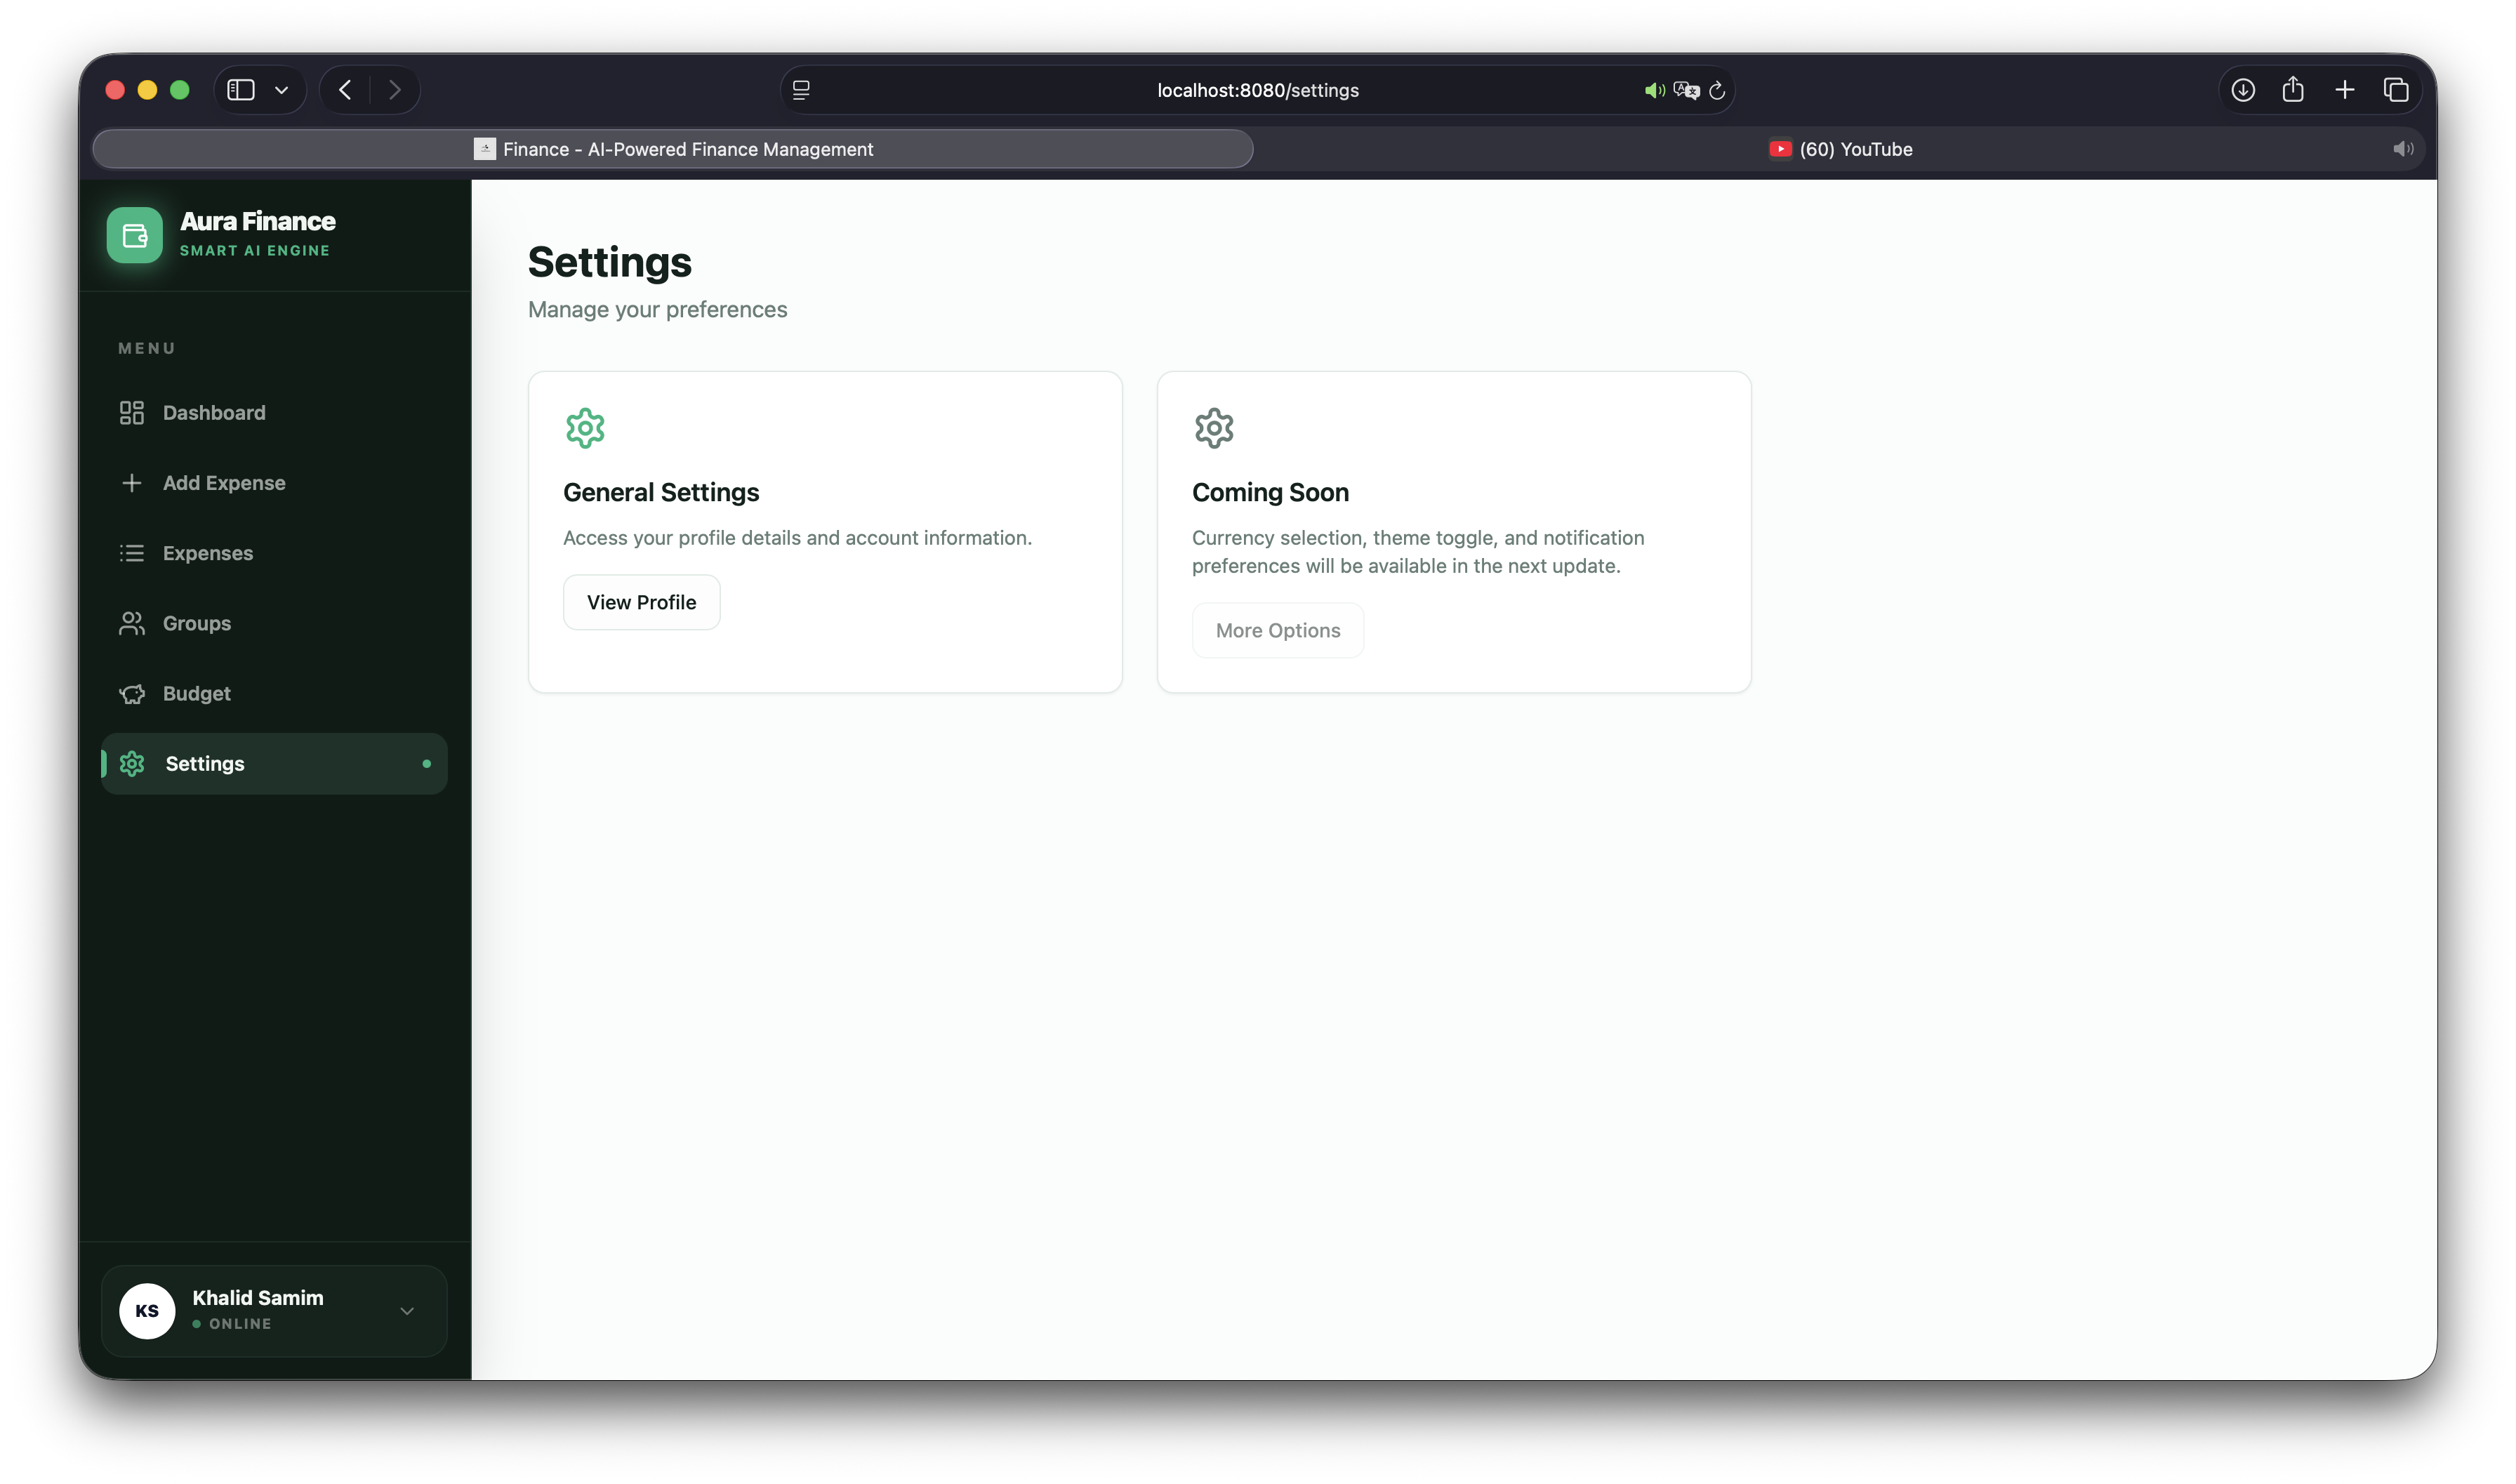
\includegraphics[width=0.8\textwidth]{./fig/aura_sc10}
 \caption{LSTM Tabanlı Gelecek Ay Harcama Tahmin Grafiği.}
 \label{fig:sc10}
\end{figure}

\subsection{Bütçe Optimizasyon Önerileri}
Şekil~\ref{fig:sc9}'da sunulan arayüz, hibrit dürtme algoritması tarafından hesaplanan "İdeal Bütçe" önerilerini gösterir. Bu öneriler, kullanıcının gelirine ve geçmiş alışkanlıklarına göre dinamik olarak şekillenir.

\begin{figure}[h!]
 \centering
 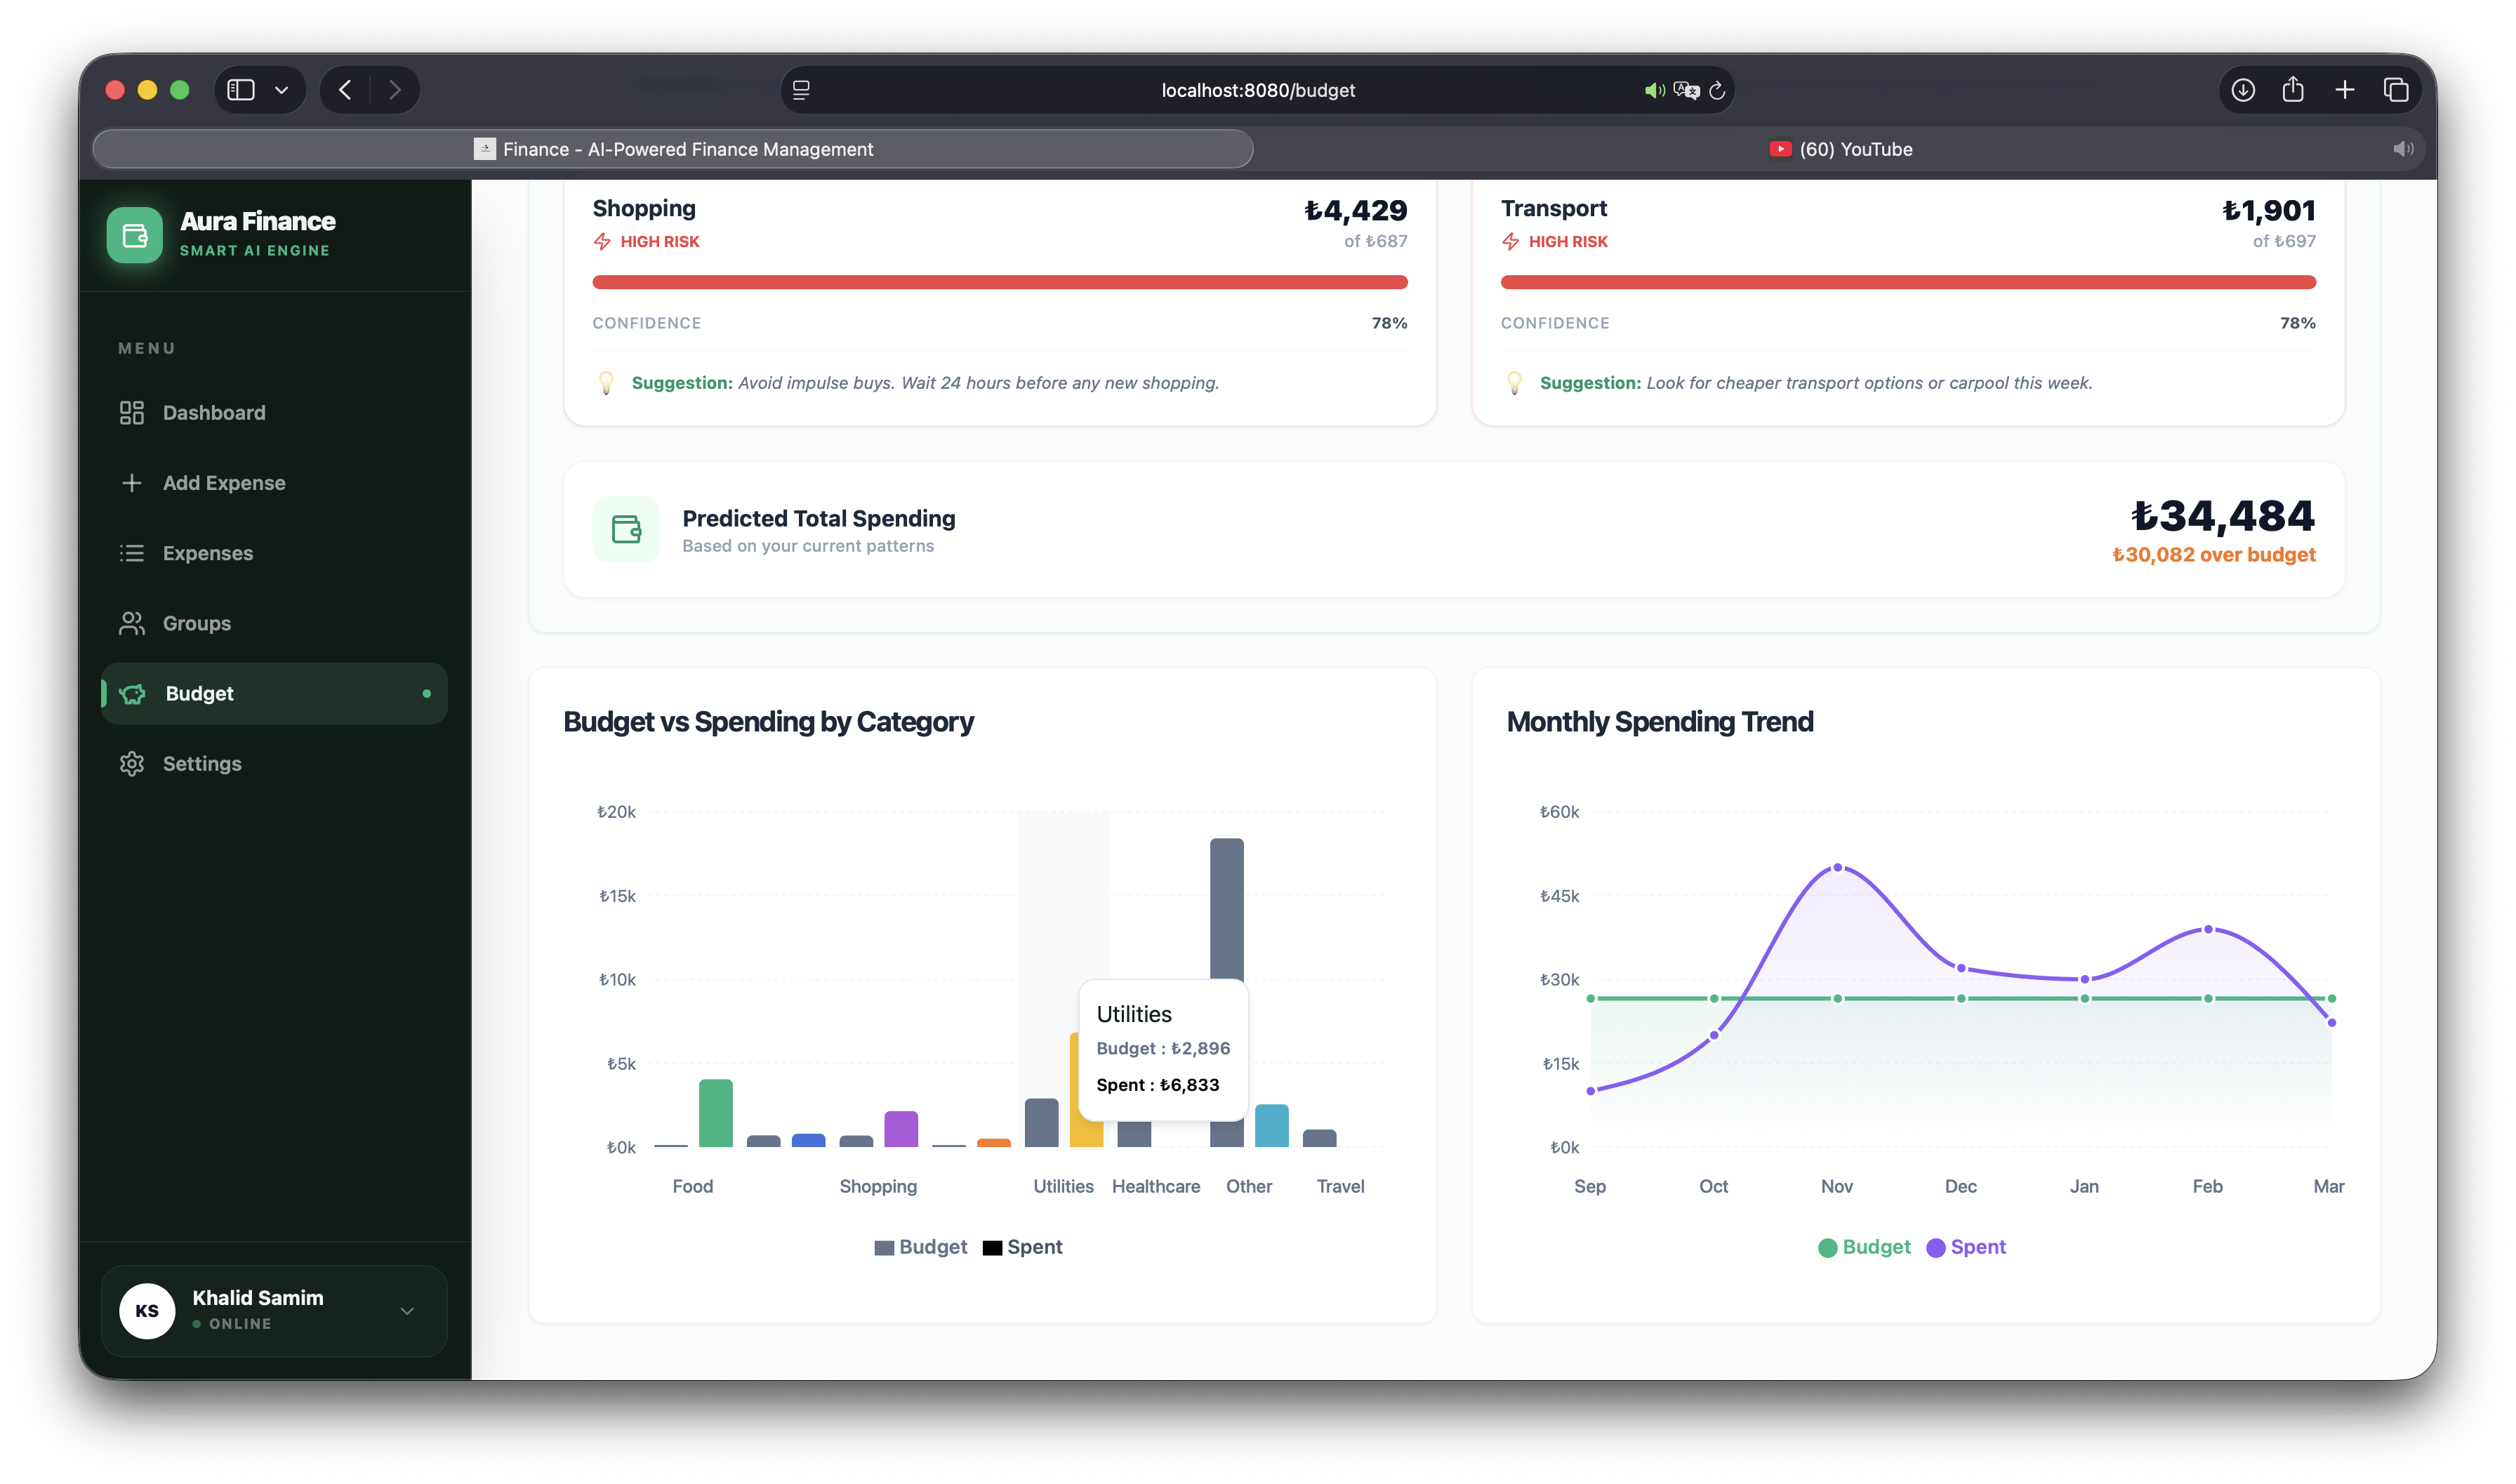
\includegraphics[width=0.8\textwidth]{./fig/aura_sc9}
 \caption{AI Destekli Bütçe Optimizasyon Önerileri.}
 \label{fig:sc9}
\end{figure}

\section{Akıllı Veri Giriş Testleri}

OCR ve Sesli giriş özellikleri farklı veri setleriyle test edilmiştir.

\subsection{OCR Başarımı}
Şekil~\ref{fig:sc5}'te bir market makbuzunun taranması ve verilerin otomatik olarak forma aktarılması gösterilmiştir. Karmaşık makbuzlarda dahi toplam tutar tespiti yüksek doğrulukla yapılabilmektedir.

\begin{figure}[h!]
 \centering
 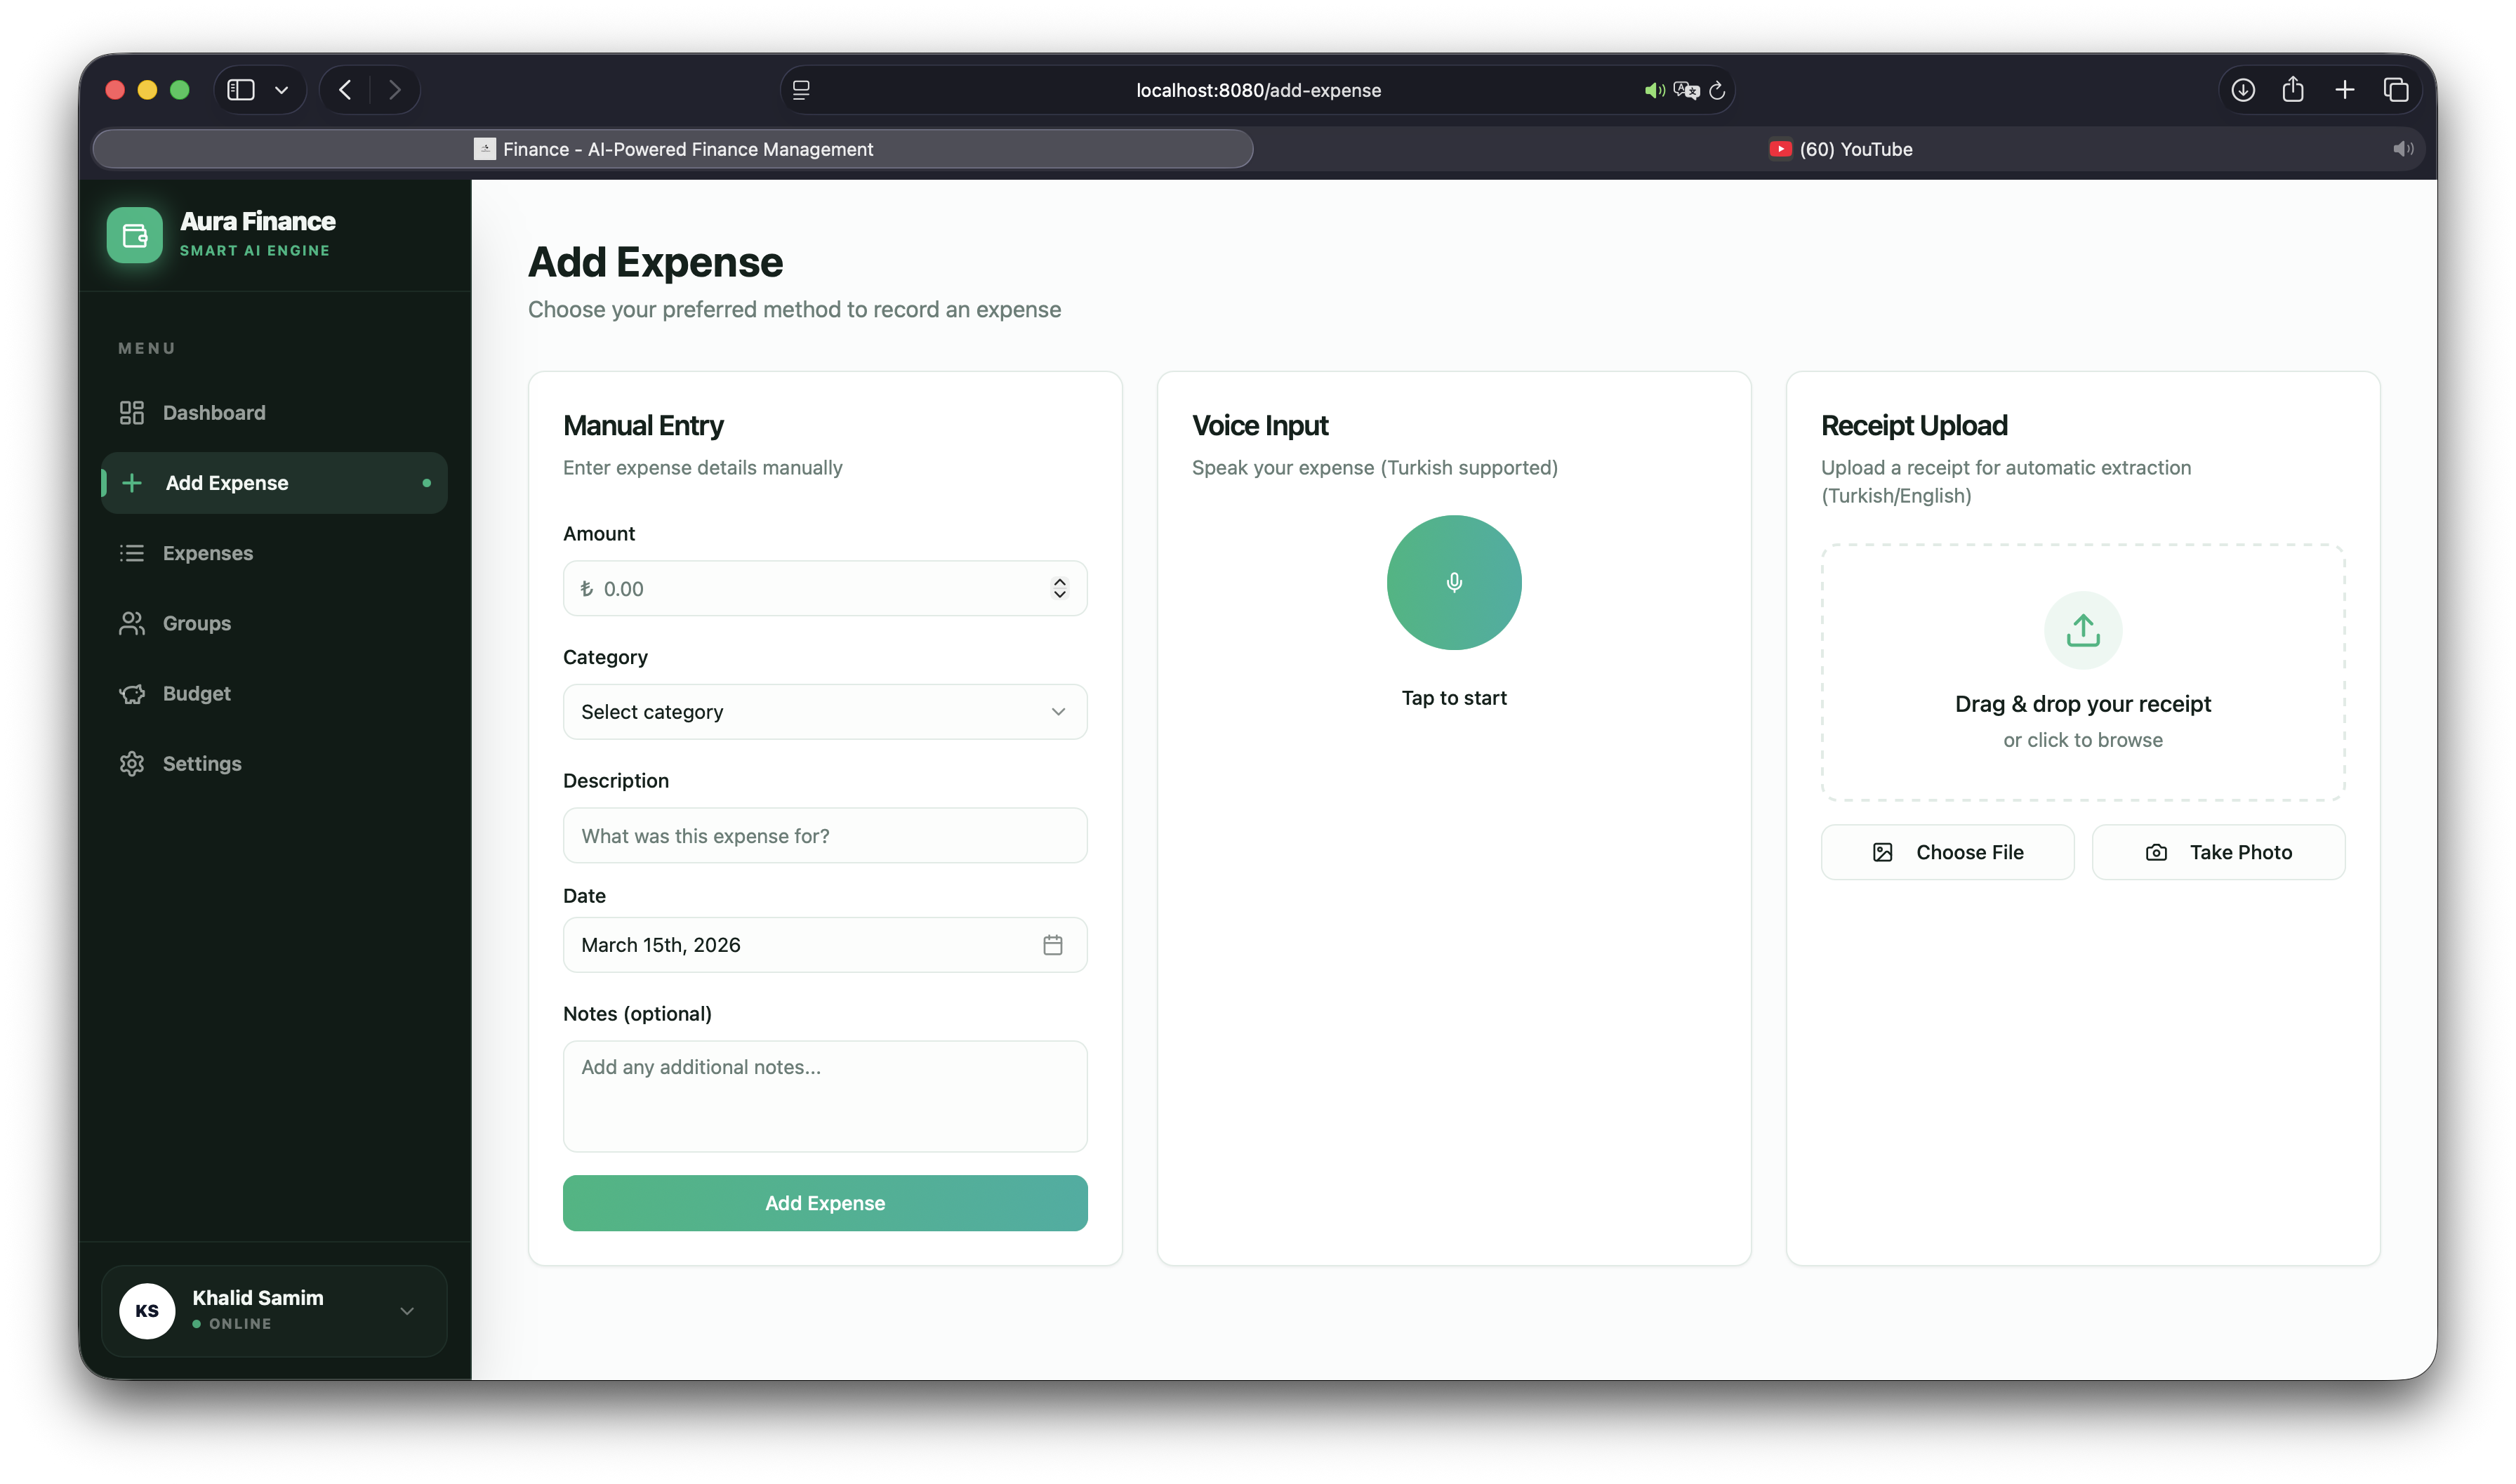
\includegraphics[width=0.6\textwidth]{./fig/aura_sc5}
 \caption{OCR ile Otomatik Makbuz Okuma Uygulaması.}
 \label{fig:sc5}
\end{figure}

\subsection{Grup Harcamaları}
Şekil~\ref{fig:sc7}, paylaşımlı harcamaların grup üyeleri arasında nasıl bölündüğünü ve takip edildiğini göstermektedir.

\begin{figure}[h!]
 \centering
 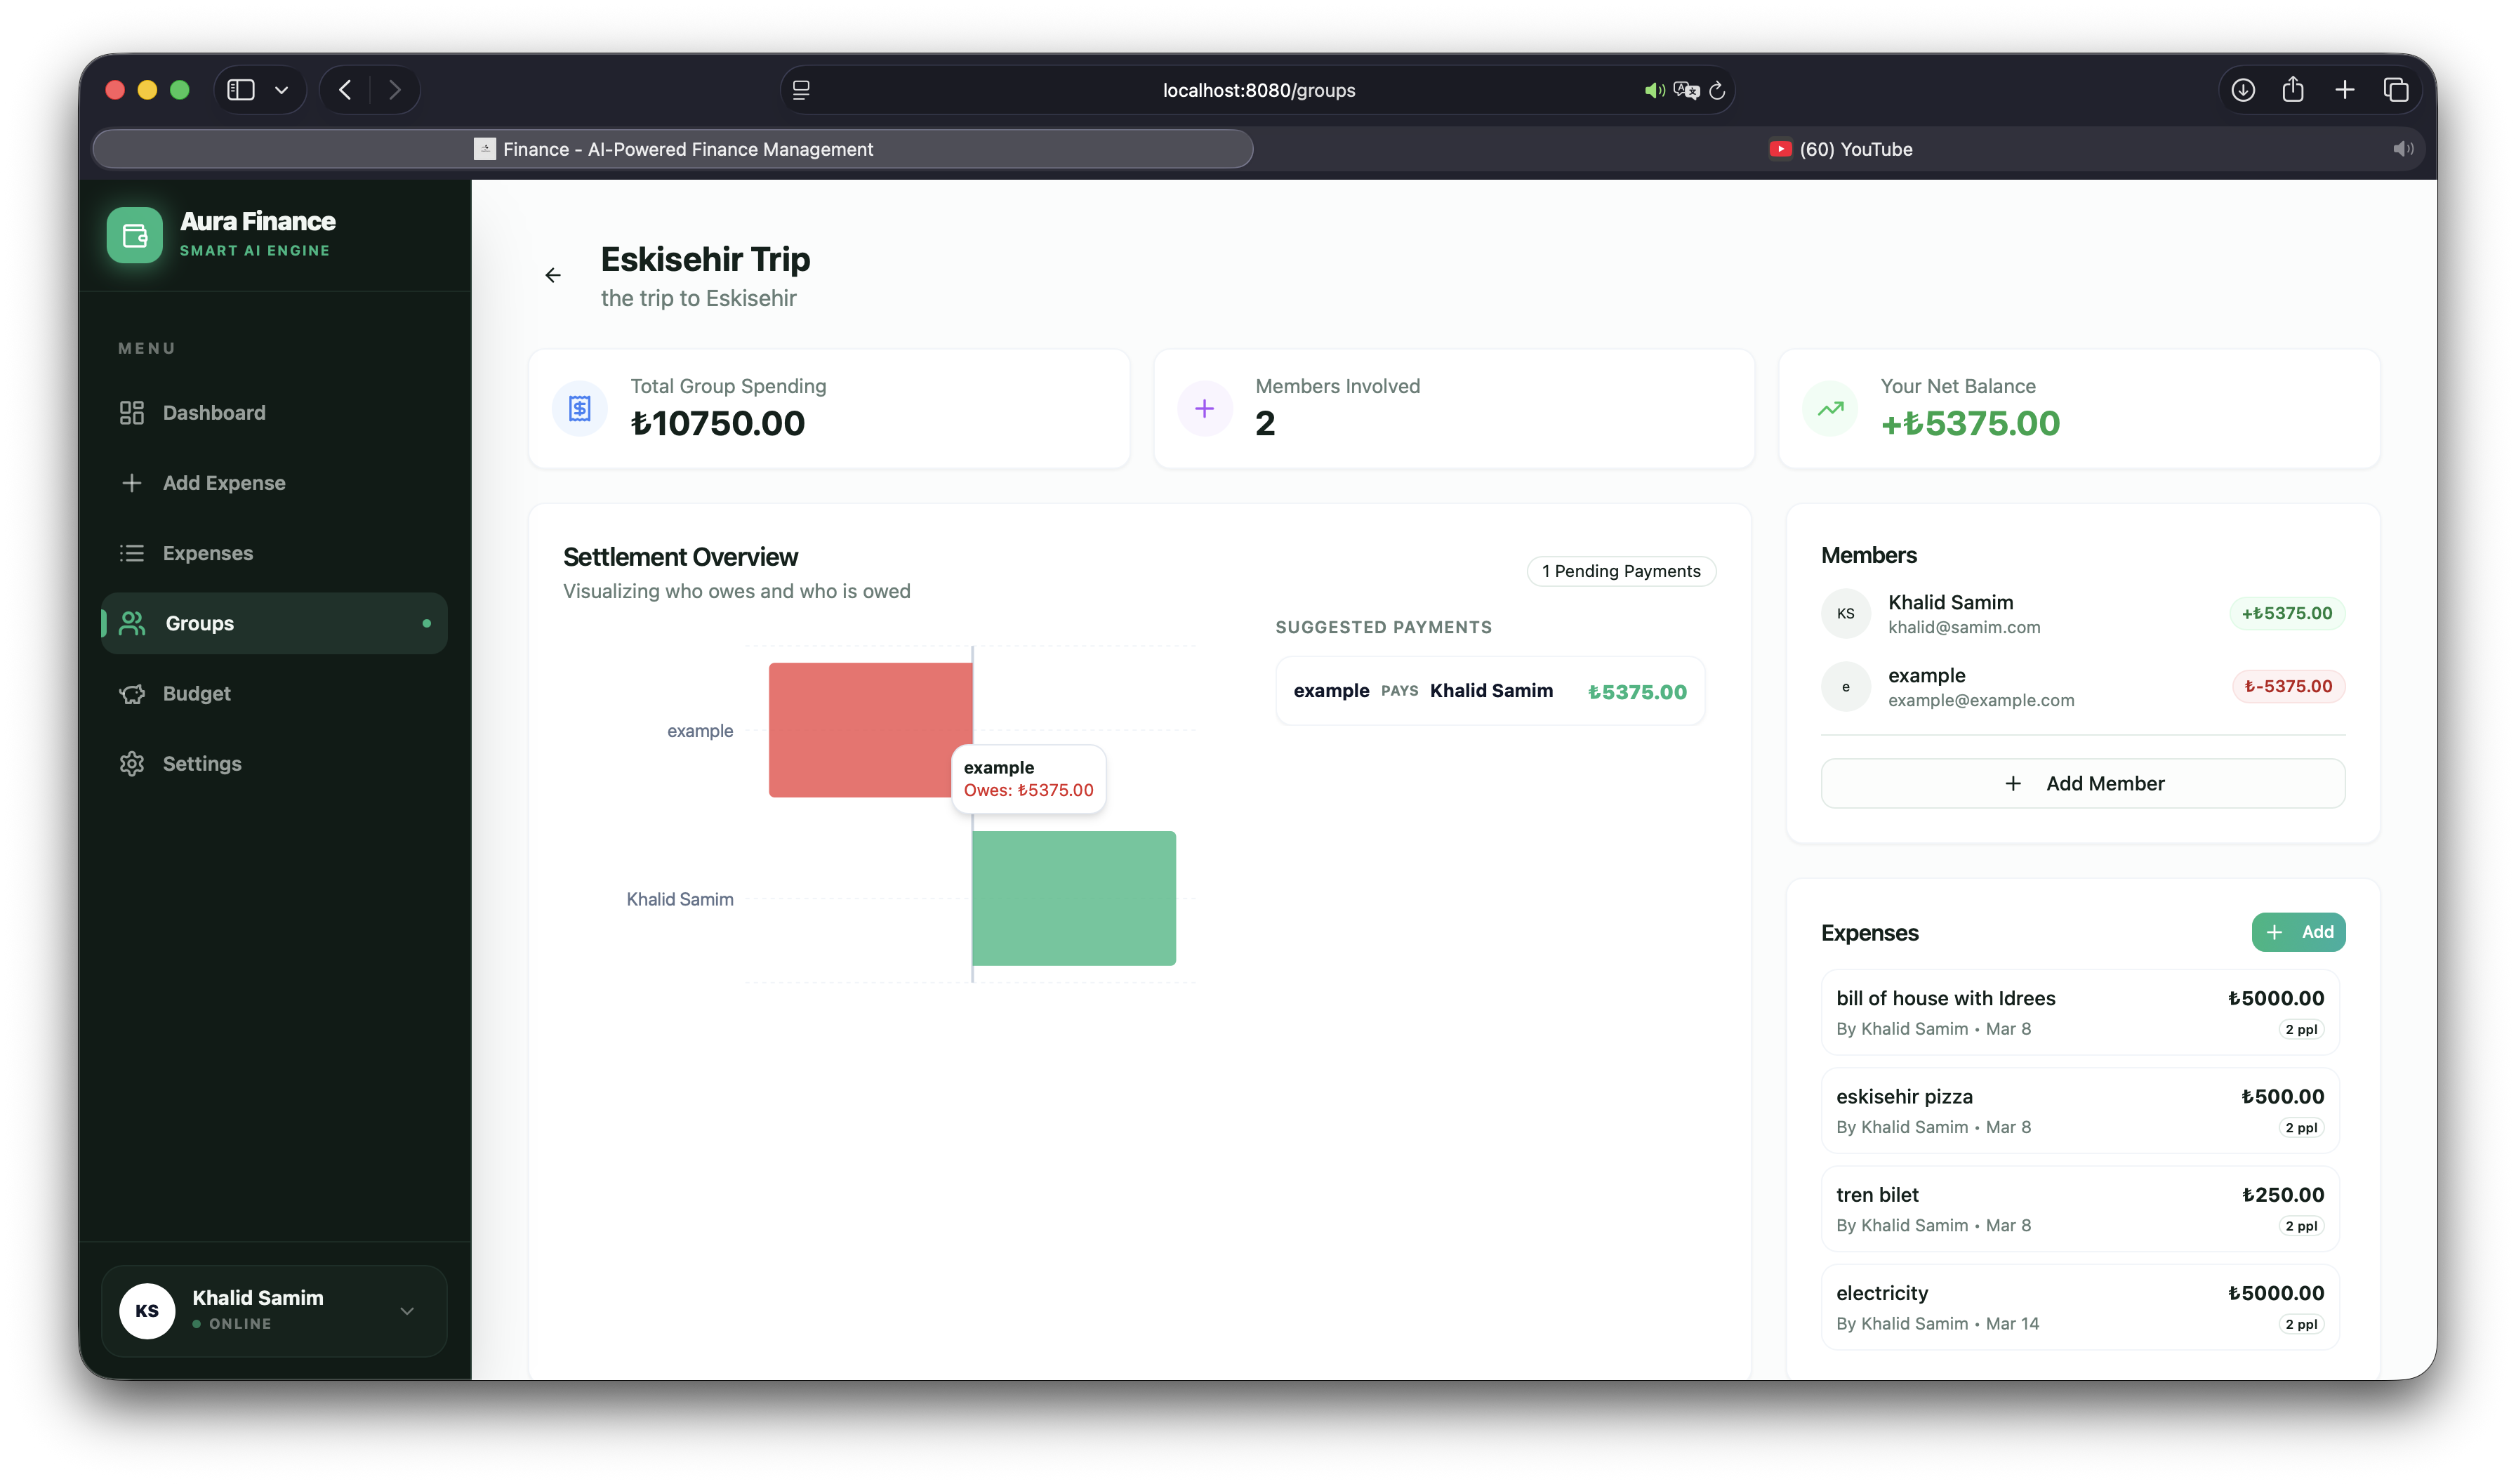
\includegraphics[width=0.8\textwidth]{./fig/aura_sc7}
 \caption{Grup Harcamaları ve Paylaşım Takip Ekranı.}
 \label{fig:sc7}
\end{figure}
